\documentclass[a4paper,oneside,article,danish,table]{memoir}
\checkandfixthelayout
\XeTeXtracingfonts= 1
\usepackage{babel,microtype,verbatim,threeparttable,amsmath,amssymb,unicode-math,hyperref,siunitx,mhchem,tikz,pgfplots,tikz-timing}
\sisetup{per-mode=symbol}
\microtypesetup{final,verbose=silent}
\usetikzlibrary{mindmap,arrows,positioning,shapes}
%\setmainfont[Ligatures={TeX}]{Arno Pro}
\setmainfont{Linux Libertine O}
\setmathfont{[Asana-Math]}
%\hfuzz=1pt
\usepackage[margin,draft]{fixme}
\fxusetheme{color}

\newcommand{\authorvar}{Carl-Emil~Grøn~Christensen \& Mathias~Dannesbo}
\newcommand{\pretitlevar}{Teknikfag~A~eksamen:}
\newcommand{\titlevar}{Swagway} 
\newcommand{\subtitlevar}{0} 
\newcommand{\datevar}{\today} 
\newcommand{\subjectvar}{Teknikfag~A:~El}
\newcommand{\classvar}{EUC~Nord: HTX~Frederikshavn, f11htx3.B}
\newcommand{\teachervar}{Alan~Gilarska}

\makepagestyle{articlehead}
\makeevenhead{articlehead}{}{\titlevar}{}
\makeevenfoot{articlehead}{}{\thepage}{}
\makeoddhead{articlehead}{}{\titlevar}{}
\makeoddfoot{articlehead}{}{}{\thepage}
\pagestyle{articlehead}

\usepackage{listings,textcomp}
\lstset{language=[Visual]C++,
  morekeywords={[2]abs,acos,asin,atan,atan2,ceil,constrain,cos,degrees,exp,floor,log,map,max,min,radians,random,randomSeed,round,sin,sq,sqrt,tan,bitRead,bitWrite,bitSet,bitClear,bit,highByte,lowByte,analogReference,analogRead,analogWrite,attachInterrupt,detachInterrupt,delay,delayMicroseconds,digitalWrite,digitalRead,interrupts,millis,micros,noInterrupts,noTone,pinMode,pulseIn,shiftIn,shiftOut,tone,Serial,Serial1,Serial2,Serial3,begin,end,peek,read,print,println,available,flush,setTimeout,find,findUntil,parseInt,parseFloat,readBytes,readBytesUntil},
  keywordstyle={\bfseries\color[rgb]{0,0,1}},
  keywordstyle={[2]\bfseries\color[rgb]{0.8,0.33,0}},
  identifierstyle=\ttfamily,
  commentstyle=\color[rgb]{0.133,0.545,0.133},
  stringstyle=\color[rgb]{0.627,0.126,0.941},
  showstringspaces=false,
  basicstyle=\small\ttfamily,
  numberstyle=\footnotesize,
  numbers=left,
  stepnumber=1,
  numbersep=10pt,
  tabsize=2,
  breaklines=true,
  breakatwhitespace=false,
  upquote=true,
  extendedchars=true,
  literate={æ}{{\ae}}1
    {ø}{{\o}}1
    {å}{{\aa}}1
}

\newcommand{\swino}[2]{\lstinputlisting[firstnumber=#1,firstline=#1,lastline=#2]{../Software/swagway/swagway.ino}}
\newcommand{\adxlh}[2]{\lstinputlisting[firstnumber=#1,firstline=#1,lastline=#2]{../Software/swagway/ADXL345.h}}
\newcommand{\adxlc}[2]{\lstinputlisting[firstnumber=#1,firstline=#1,lastline=#2]{../Software/swagway/ADXL345.cpp}}
\newcommand{\itgh}[2]{\lstinputlisting[firstnumber=#1,firstline=#1,lastline=#2]{../Software/swagway/ITG3200.h}}
\newcommand{\itgc}[2]{\lstinputlisting[firstnumber=#1,firstline=#1,lastline=#2]{../Software/swagway/ITG3200.cpp}}
\newcommand{\boarddate}[1]{\marginpar{\textcolor{blue!80!black}{#1}}}
\newcommand{\issue}[1]{\textsuperscript{\textcolor{blue!80!black}{\href{https://github.com/neic/Swagway/issues/#1}{\##1}}}}


\begin{document}
% \includepdf{forside.pdf} \clearpage%------------------------ Forside

\noindent
{\fontsize{90}{108}\selectfont \color{red!80!black}\titlevar}\\
\vfill
\noindent
{\color{blue!90!black} \LARGE
{\fontsize{16.55}{20}\selectfont \authorvar}\\
\begin{tabular*}{\textwidth}{@{\extracolsep{\fill}} ll}
  \subjectvar & \datevar\\
\end{tabular*}
}

\thispagestyle{empty}
\clearpage
\begin{center}
  \if\pretitlevar 0
  \else{\Large\pretitlevar\\} \fi
  \textsc{\HUGE\titlevar\\}
  \if\subtitlevar 0
  \else {\Large\subtitlevar\\} \fi
  %\vspace{1em}
  {\LARGE 
  af\\
   \authorvar}\\
\end{center}

\vfill
\begin{abstract} %------------------------------ Abstract
  \fxwarning{Skriv resume}
\end{abstract}\vfill
\noindent
\begin{tabular*}{\textwidth}{@{\extracolsep{\fill}} ll}
  \classvar&\subjectvar\\
  {Lærer: }\teachervar & \datevar\\
\end{tabular*}
\thispagestyle{empty}
\clearpage

\chapter*{Forord}\label{chap:for}
Gennem teksten vil der være angivet link til “Issues” på GitHub siden for projektet.\footnote{\url{https://github.com/neic/Swagway}} Disse Issues har været brugt som projektstyring samt bugtracker igennem projektforløbet. Links er angivet som i enden af denne sætning.\issue{1} Det er ikke nødvendigt for forståelsen af denne rapport at følge linksne.

Vi vil gerne takke Steffen Linnerup Christiansen for hjælp med mekanikken, samt Kristian Holm Nielsen for hjælp med forståelsen af PID.

\clearpage \setcounter{tocdepth}{1} \tableofcontents \clearpage

\chapter{Indledning}\label{chap:ind}
Transport enheder bliver mere og mere avancerede, og der skabes ofte nye enheder. Specielt mobilitet og anvendelighed har været i højsædet i mange nye produkter. Det handler om hurtigt at kunne komme fra punkt a til punkt b, uden at det kræver større besvær. Derudover er løsninger som er intuitive at bruge også fremskreden, og et produkt som opfylder alle disse punkter er Segwayen. Den er hurtig, kræver næsten ingen erfaring at køre på og er lille. Man kan hurtigt suse fra en afdeling til anden. 

Formålet med projektet er at bygge en motoriseret selvbalancrende tohjulet transportenhed. Det er en klon af en Segway som er et kommercielt produkt, der benyttes af en lille skare af befolkningen nutildags. Kendetegnet ved Segwayen er, at de to hjul sidder på samme aksel, hvor elektronik og motorene sørger for at, selv med en fører, holde enheden i balance.
\begin{figure}[htbp]
  \centering
  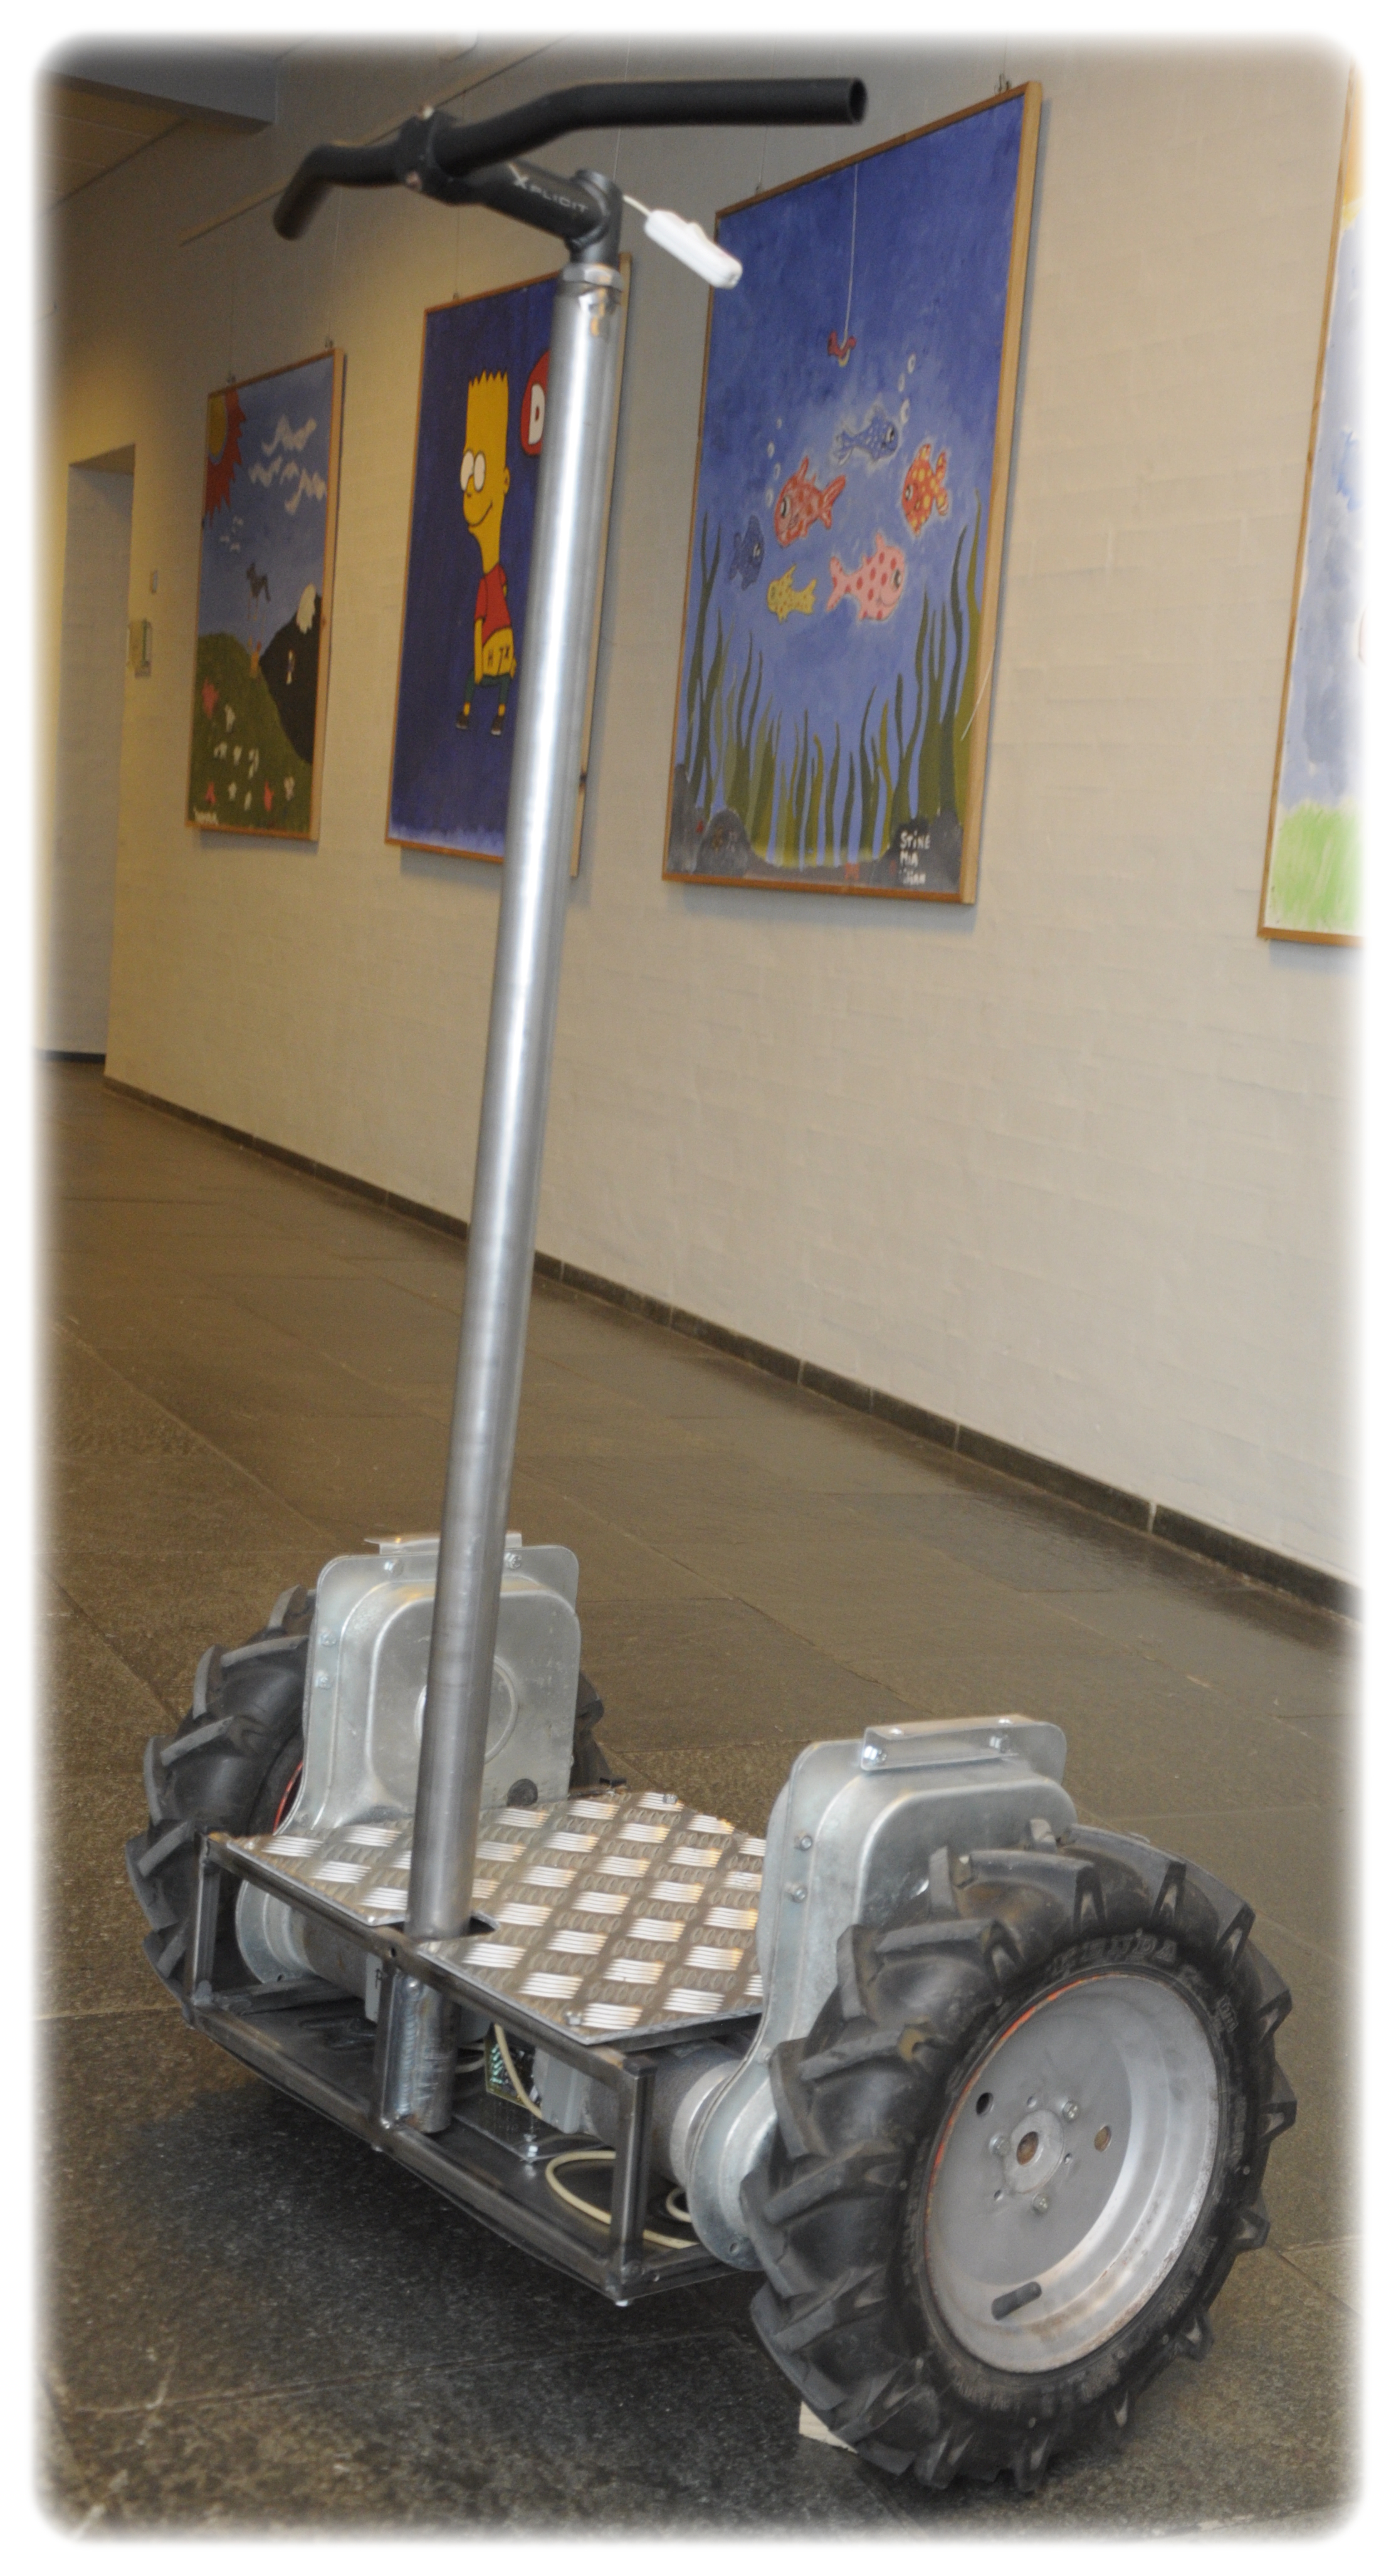
\includegraphics[width=0.4\textwidth]{pictures/swagway.jpg}
  \caption{Den mekaniske udformning af Swagway}
  % \label{fig:}
\end{figure}
Når en fører læner sig frem eller tilbage, kompenserer Segwayen ved køre i samme retning, for atter at balancere den. For at dreje enheden vipper føreren håntaget til den ene eller anden side, som man ønsker at dreje til. Segwayen kan købes for cirka halvfjerdstusinde kroner, hvis man ønsker at eje sådan en.

Projektoplæget lyder:
\begin{quote}
  Formålet er at bygge en balance robot på to hjul, en Segway klon. Minimums målet er at få robotten til at balancere. Derefter få den til at køre og kunne styre den hvis tid og evner rækker til det.
\end{quote}

Hovedeudfordringen er at holde enheden lodret. For at gøre dette skal man kende enhedens vinkel i forhold til lodret og omsætte denne vinkel til et signal til motorene. Når vinklen stiger driver motorene hjulene som så flytter enheden og brugerens tygdepunk ind over akslen igen.
Det kan se som tre isolerede problemstillinger som passer ind i I-C-O-modellen:
\begin{itemize}
\item[Input] Måle Swagwayens hældning i forhold til lodret
\item[Control] Omsætte vinklen til et signal til motorene.
\item[Output] Drive to motore baseret på signalet.
\end{itemize}

Projektet er udarbejdet ud fra mikrokontrolleren Arduino Uno, i programmet arduino. Mikrokontrolleren bliver programmeret via. programmet Arduino, som nærmest er i sproget C++ med et Arduino bibliotek. Da vi har modtaget undervisning i denne platform, har dette været det oplagte redskab at benytte til løsningen af vores projekt.

\chapter{Input}
\section{Sensor}
Efter nogen research af andre køretøjer og mindre robotter med der fungerer på sammen måde, var det klart at gyroskoper og accelerometere kunne måle vinklen så hurtigt og præcist som det var krævet.
\subsection{Sensor hardware}
Gyroskoper og accelerometere har indtaget forbrugerens produkter, og kortlægger allerede nu deres bevægelser. De faldende priser og faldene energiforbrug har gjort, at gyroskoper og accelerometere er langt mere tilgængelige for alle. Mobiltelefoner, spilkonsoller og kameraer kan nu måle hvordan du bevæger dig, og flere og flere enheder importerer også disse bevægelses sensorer, for at adskille sig fra de andre.

Disse bevægelses sensorer er avancerede MEMS (mikroelektromekaniske systemer) teknologier, som inkoorpererer gyroskoper, accelerometere og kompas sensorer. % Bevægelses behandling foretages oftest med en kombination af to sensorer, for at få optimal præcision.
I dette projekt har vi arbejdet med gyroskoper og accelerometere, som vi også kender fra vores smartphones. Swagwayen skal, lige som en smartphone kan måle om den står eller ligger ned, måle i hvilken vinkel den står i. \fxnote{Check om vi har forklaret at der er brug for begge komponenter}  

\subsubsection{Gyroskop}
Et gyroskop måler vinkelhastigheder, hvor hurtigt noget drejer om en akse. Hvis denne vinkelhastighed integreres over tid finder man vinklen som gyroskopet har flyttet sig. Problemet med at integrer gyroskopdata er, at pga. måleusikkerheder vil det målte nulpunkt drive væk fra det fysiske nulpunkt. Moderne gyroskoper er et mikroelektromekanisk system, også kaldet MEMS. Det betyder, at det både er en mekanisk og elektrisk funktion i et system. /fxnote{hvordan fungerer MEMS i et gyroskop}

\subsubsection{Accelerometer}
Et accelerometer kan måle accelerationer. Man kan med hjælp fra tangens og data fra to akser udregne den vinklen accelerometeret står i forhold til jordens tyngdekræft. Problemet med dette er at accelerometer måler alle accelerationer, ikke kun jordens tyngdekræft. Når Swagwayen fx accelerer, bremser eller køre over en sten bliver den udregnet vinkel forkert.
\begin{figure}[htbp]
  \centering
  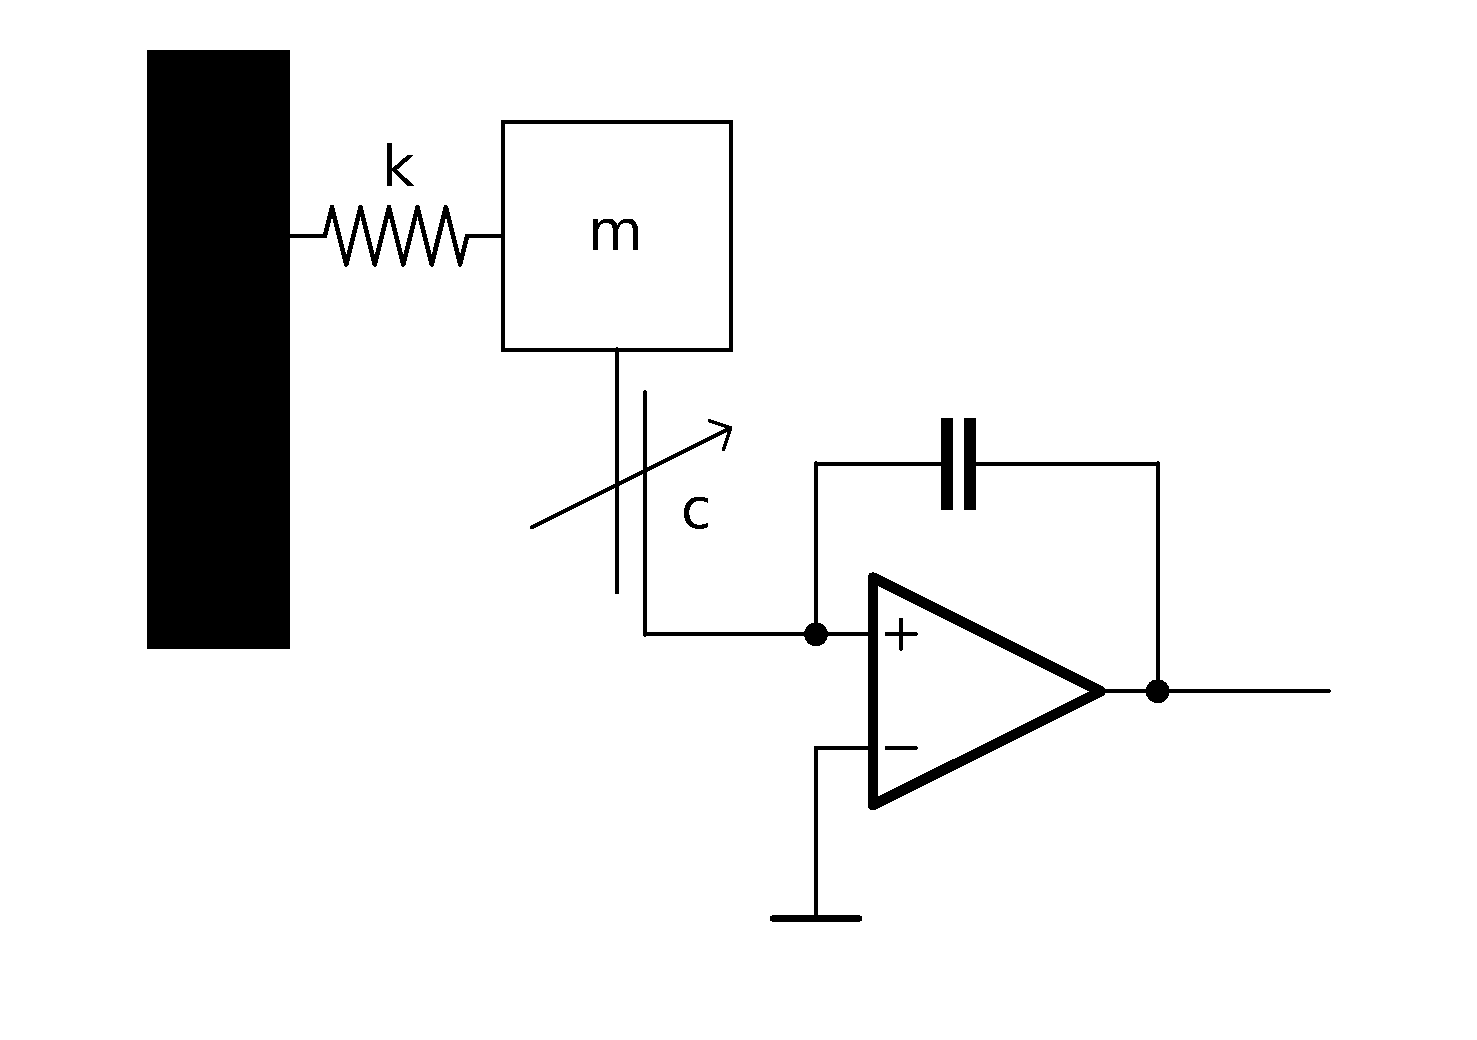
\includegraphics[width=\textwidth]{pictures/accbasic.pdf}
  \caption{Et accelerometers interne MEMS-struktur}
  \label{fig:memsacc}
\end{figure}
Et accelerometer måler en bevægelse, som enten er forårsaget af tyngdekraften eller en bevægelse. Som set på figur \ref{fig:memsacc} måles accelerationen i et moderne MEMS accelerometer ved en ændring i kapacitansen, $c$, som skyldes en ændring i massens, $m$, position. Kapasitansen fører til en ændring i spændingen, som herefter digitaliseres via ADC og kan benyttes af en mikrokontroller som Arduinoen. Dette gøres for de tre akser x, y og z, og accelerationen kan nu måles i alle retninger.

\subsubsection{IMU}
For at løse problemet med at gyroskopet driver og problemet med at accelerometret ikke er nøjagtig når det bliver påvirket af andre accelerationer end tygdekraften kan man bruge begge sensorer sammen. Man bruger begge sensoreres data og samler dem i et filter. Se mere herom i sektion \ref{sec:filter}.

De fleste moderne accelerometere og gyroskoper kommer i små SMD pakker som er vanskelig håndlodde. Heldigvis er det forholdsvis let at få disse sensorer monteret på et breakoutboard. Efter at have kigget på andre Segway kloner og balancerobotter faldt valget på en IMU fra Sparkfun. Se figur \ref{fig:imu}. En inertial measurement unit, IMU, er en enhed som kombinere flere sensorer.
\begin{figure}[htbp]
  \centering
  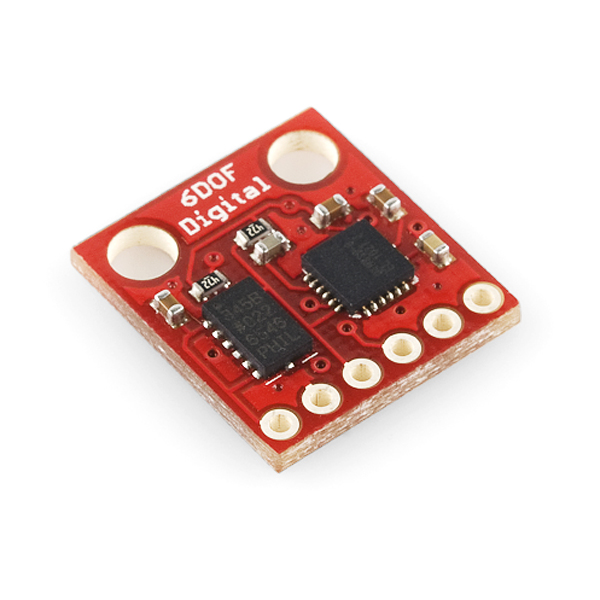
\includegraphics[width=0.3\textwidth]{pictures/imu.jpg}
  \caption[6DOF IMU breakoutboard fra Sparkfun]{6DOF IMU breakoutboard fra Sparkfun. (CC BY-NC-SA 3.0, Sparkfun)}
  \label{fig:imu}
\end{figure}
IMUen fra Sparkfun et ADXL345 accelerometer og et ITG-3200 gyroskop. Accelerometret og gyroskopet er begge tre-akset. \fxnote{tre-akset?} Det giver IMUen seks frihedsgrader (DOF). Swagwayen skal dog kun bruge tre frihedsgrader; to akser fra accelerometret og en fra gyroskopet, men IMUen med seks frihedsgrader var det mindste med digital interface.

\subsection{I²C}
Kommunikation med IMUen sker digital over en I²C-bus. På bussen er der en master\footnote{Det er mulig at lave et multi-master opstilling hvis alle masterne understøtter det.} og en eller flere slaves. I Swagwayen er Arduinoen master og accelerometeret og gyroskopet er begge slaves. I²C bussen består af to fysiske forbindelser, en serial data linje (SDA) og en clock (SCL). Alle enheder på bussen forbinder til disse to forbindelser. Linjerne er open-drain med eksterne pull-up modstande. Det vil sige at i hver enhed sidder der MOSFETer der trækker spændingen på linjen mod GND efter behov. De eksterne pull-op modstande trækker linjerne op igen. Se figur \ref{fig:i2cbasic}.
\begin{figure}[htbp]
  \centering
  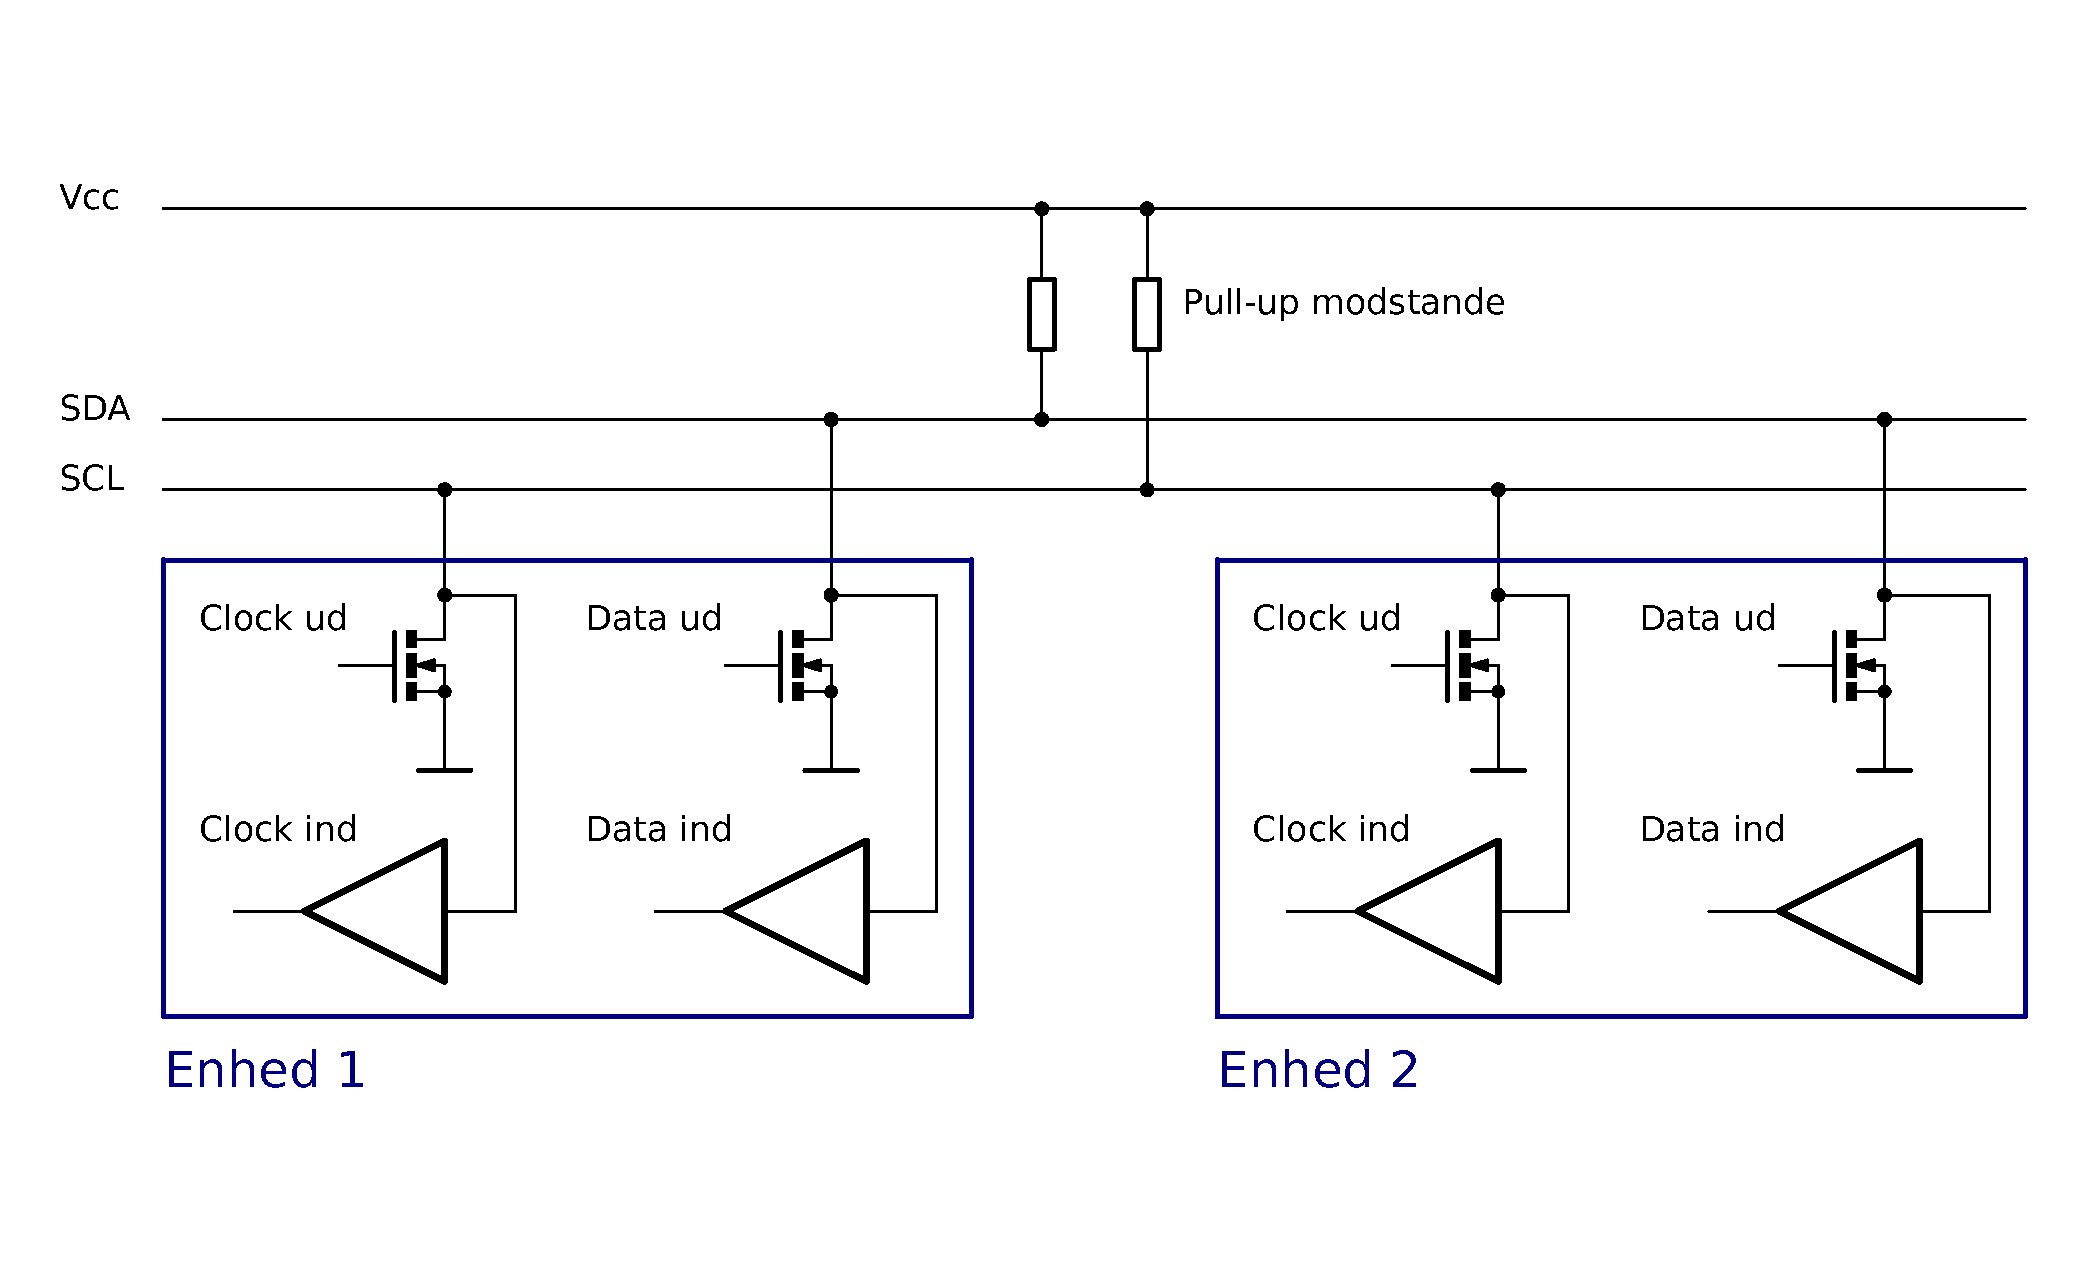
\includegraphics[width=\textwidth]{pictures/I2Cbasic.pdf}
  \caption{Eksempel på I²C-netværk}
  \label{fig:i2cbasic}
\end{figure}

På Arduinoen er I²C SDA på A4 og SCL på pin A5 med indbygget pull-up modstande på \SI{20}{k\ohm}--\SI{50}{k\ohm}. \cite[s. 317]{atmega} De er aktiveret som standard når man bruger Wire biblioteket.\footnote{For reference se linje 75 i \texttt{utility/twi.c} i Wire biblioteket.}

Arduinoens spænding er \SI{5}{V} og IMUens er \SI{3,3}{V}. IMUen bliver forsynet med \SI{3,3}{V} fra Arduinoen, men SDA og SCL er koblet direkte til Arduinoens pins som har \SI{5}{V} som reference. Den korekte løsning ville være at lave en level-shifter imellem en \SI{5}{V}- og en \SI{3,3}{V}-del af I²C-bussen, men når pull-up modstandene er så høje som de er det stadig forsvarligt at kører IMUen direkte med \SI{5}{V} som $V_{IO}$-reference. Der er flere eksempler på det samme blandt andre på Internettet der bruger samme chips.

Den lætteste måde at kommunikere over I²C fra en Arduino er at bruge Wire-bibliotektet som kommer sammen Arduino-softwaren: \lstinline{#include <Wire.h>} For at få Arduinoen til at tilslutte sig bussen som master kaldes \lstinline{Wire.begin();} uden parametere. Slaverne på I²C-bussen har alle en adresse som fremgår af deres respektive datablade.

ADXL345 og ITG-3200 indeholder begge flere register med forskellige funktioner. Nogle registre indeholder opsætningen for chippen, andre indeholder det data som chippen måler. Hvis man, fra Arduinoen, vil skrive til et af registrene køre man følgene kode:
\begin{lstlisting}
  Wire.beginTransmission(deviceAddress);   // begynder en session med enheden med deviceAddress
  Wire.write(regAddress); // sender adressen på den register man vil ændre
  Wire.write(value); // sender værdien registeren skal indtage
  Wire.endTransmission(); // afslutter sessionen
\end{lstlisting}

At læse et register er lidt mere omfattende:
\begin{lstlisting}
 Wire.beginTransmission(deviceAddress); // begynder en session med enheden med deviceAddress
 Wire.write(regAddress); // sender adressen på den register man vil ændre
 Wire.endTransmission(); // afslutter sessionen
  
 Wire.beginTransmission(deviceAddress); // begynder en ny session
 Wire.requestFrom(deviceAdress, numberOfBytes); // sender anmodning på at modtage numberOfBytes
 int i = 0; 
 while (Wire.available()) { // så længe der er data tilgængeligt
   buffer[i] = Wire.read(); // modtag data og fyld det i buffer
   i++;
 }
 Wire.endTransmission(); // afslutter sessionen
\end{lstlisting}

Disse to funktioner bliver senere refereret til som hhv. \lstinline{writemem()} og \lstinline{readmem()}.

\fxwarning{skriv om hvad registerne kan}

\subsection{IMU biblioteker}
I begyndelsen af projektet var alt kommunikationen med ADXL345 og ITG-3200 programmeret i \texttt{swagway.ino}. Det virkede og Arduinoen modtog data fra IMUen, men koden var svær at vedligeholde og gik tit i stykker. Der var desuden en fejl igennem lægere tid der resulterede i at den vinkel der blev udregnet fra gyroskopet, \lstinline{gyroAngle}, var ca. dobbelt så stor som den burde være.\issue{20} Efter mange ufuldendte forsøg på at rette fejlen blev alt gammel kode der var releateret til I²C slettet. Der blev istedet brugt et bibliotek passende til gyroskopet hvor alle funktioner var implementeret. Biblioteket hedder itg3200.

Det var ikke til at finde et ligende bibliotek til accelerometret, så med inspiration fra itg3200-bibliotekt blev der skrevet et. Biblioteket består af to filer. En headerfil, \texttt{ADXL345.h}, og selve funktionaliteten, \texttt{ADXL345.cpp}.

Headerfilen indeholder først definitioner på konstanter som enhedsadressen og registere:
\adxlh{23}{35}
Værdierne og navnene er hentet fra \cite[s. 23]{adxl345} At have definitioner på alle konstanter gør koden lættere læselig, så man ikke skal søge referencer i databladet.

Efterfølgene er der defineret en klasse med alle funktioner relateret til accelerometeret:
\adxlh{37}{49}

I \texttt{ADXL345.cpp} er funktionalitet skrevet. Som eksempel er her tre af de første funktioner er begge til opsætning af accelerometret.

\subsubsection{setMeasureMode()}

\adxlc{33}{36}
\lstinline{setMeasureMode()} skriver til power control registret, \lstinline{POWER_CTL}. Funktionaliteten af \lstinline{POWER_CTL} er beskrevet i \cite[s. 25--26]{adxl345}. \lstinline{POWER_CTL}s adresse er, som tidligere beskrevet, defineret i \texttt{ADXL345.h}. \lstinline{MEASUREMODE} er en sekvens af otte bits (en byte) somm hvis de skrives i \lstinline{POWER_CTL}, vil sætte accelerometret i måle tilstand. Sekvensen er ligledes udledt af \cite{adxl345}. Den er i dette tilfælde \texttt{0000\,1000}.

\subsubsection{getOutputRate()}

\adxlc{38}{42}
\lstinline{getOutputRate()} læser registret \lstinline{BW_RATE}, ligger dataene i en buffer og retunerer aflæsningen.

\subsubsection{setFullRes()}

\adxlc{56}{60}
\lstinline{setFullRes()} skal kun ændre \emph{en} bit i registret \lstinline{DATA_FORMAT}. For at bebeholde de andre bits læser den først det som står i registret og gemmer det i en buffer. \lstinline{1 << 3} betyder en bit shiftet tre pladser til venstre: \texttt{0000\,1000}.  \lstinline{~(1 << 3)} er Bitwise NOT værdien af dette: \texttt{1111\,0111}. Det bliver AND med bufferen, \lstinline{(_buff[0] & ~(1 << 3))}. Det er lig med alle de bit som er sat i bufferen pånær den fjerde sidste. Altså: den sætter den fjerde sidste bit til 0 og bibeholder alle andre. \lstinline{(_fullRes << 3)} er værdien der skal sættes shiftet tre pladser til venstre: \texttt{0000\,x000}. Disse to værdi bliver til slut OR med hindanden og den fjerde sidste bit er nu ændret til værdien af \lstinline{_fullRes} uden at nogle andre bits bliver ændret. Denne værdi bliver nu skrevet tilbage i samme buffer.

To andre eksempler på funktionaliteten af \texttt{ADXL345.cpp}. Disse funktioner har med modtagelse af data at gøre.

\subsubsection{isRawDataReady()}
\adxlc{75}{79}
Accelerometeret har et register med interrupt flag, \lstinline{INT_SOURCE}. \lstinline{isRawDataReady()} læser dette register og gemmer det i en buffer. Bufferen bliver shiftet syv pladser til højre og  \lstinline{isRawDataReady()} retunere en bool værdi alt efter om interrupt flaget er sat.

\subsubsection{readAccRaw()}
\adxlc{99}{105}
Dataende i accelerometeret fylder seks registre af 8 bit. Hver akse fylder to registre hvoraf det første er den mindst betydene. \lstinline{readAccRav()} læser \lstinline{DATAX0} og seks registre frem. Dataene bliver lagt i et buffer-array. Den mest betydene af de to bytes som høre sammen bliver shiftet 8 pladser til venstre og derefter AND med den mindst betydene. De to bytes bliver sat sammen direkte efter hindanden. Værdierne bliver retuneret til tre integer-pointers.

\section{Styring}
Styringen af Swagwayen skulle være en længerevarende og holdbar løsning. Det ønskes ikke, at enheden efter forholdsvis kort tid skulle udskiftes eller repareres. Vi overvejede fem forskellige løsninger: En lineær potentiometer, et drejepotentiometer, gaffelsensor, strain-gate og stepper motor.
\subsection{Lineær potentiometer} \fxnote{billede af linæert potentiometer fig:linpot}
Et lieært potentiometer fungerer som et normalt potentiometer, dog trækkes "armen" i en sliske som set på figur \ref{fig:linpot}
Potentiometret skal placeres i bunden af stangen, hvorefter potentiometrets arm trækkes med stangens bevægelse. Herefter vil man kunne ændre på PWM signalet til motorene, og på den måde dreje. Løsningen er simpel at udføre, og vil virke let i praksis.

Ulempen ved denne løsning er dog, at potentiometret hurtigt slides op ved brug, og det er derfor ikke en holdbar løsning. \fxwarning{wut?}
\subsection{Dreje potentiometer}
Samme princip fra det lineæere potentiometer gælder her. Derimod drejes dette potentiometer i stedet for om sin egen akse. Ideen med dette var, at man let kan implementere den i toppen af Swagwayens styr, og så styre PWM signalet til motorerene sådan. 

Lige som det linæere potentiometer, slides denne løsning hurtigt, og er derfor ikke holdbar. Derudover er denne løsning ikke lige så intuitiv og føles klodset, hvilket ikke er det vi ønsker med produktet.
\subsection{Gaffelsensor}
Gaffelsensorer benyttes i gamle kuglemuse, som vi alle nok kender. Gaffelsensorene måler hvor meget noget har flyttet sig ved at analysere bevægelsen i forhold til nogle bånd buede bånd, i to krysende retninger. Ud fra bevægelsen kan gaffelsensoren bestemme, hvordan kuglen har bevæget sig i dens socket. En lignende anordning kunne placeres i bunden af stangen lige som det lineæere potentiometer, og en kugle kunne skubbes rundt lige som i en mus, for at bestemme stangens hældningen. Løsningen er meget præcis hvis den er lavet mekanisk godt.

Gaffelsensoren er derimod ekstremt upræcis hvis mekanikken ikke er rentskåret-næsten perfekt. Yderligere bliver dens præcision påvirket af støv og skidt, hvilket hurtigt vil ophobe sig i bunden af vores Swagway.
\subsection{Strain-gate}
En strain-gate løsning er en anordning, som placeres på siden af stangen. Strain-gaten kan mærke tryk i metallet, og kan ud fra dette tryk bestemme en værdi, som man kan bruge til at styre Swagwayen med. Denne løsning er ekstrem præcis, og benyttes ofte i store maskiner.

Problemet er dog, at den ikke virker på vores stang, da den er for stiv, og løsningen hverken er intuitiv eller responsiv for forbrugeren. Den er ikke lige til at finde ud af fra første øjekast, og den er sværere at lære.
\subsection{Stepper motor}
Det sidste løsningsforslag: Stepper motor. Planen med denne var at foretage den modsatte funktion af hvad man normalt gør med en stepper motor: I stedet for at få motoren til at bevæge noget, skal styret bevæge motoren, hvorefter det måles hvilket step den er på i Arduinoen. Løsningen er ekstremt robust og præcis, som vi kender stepper motorer for. Derudover vil den ikke være modtagelig for omgivelsernes påvirkninger i form af støv eller andet snavs. Yderligere kan steppene geares, så den bliver endnu mere præcis hvis nødve
+ndigt.

Det sværeste ved denne løsning er, at implementere den. 

Hvis tiden havde rækket til det, havde vi derfor valgt denne som den umiddelbare løsning.
\chapter{Control}
\section{Hoved \lstinline{loop()}}
\fxerror{Skriv om main loop}
\section{Filter}\label{sec:filter}
Målet med filtret er at samle dataen fra gyroskopet, accelerometeret og ud fra disse beregne en vinkel, som vi kan benytte til at regulere PWM efter. Ud fra dette mål, udvalgte vi tre filtre, som har de egenskaber vi leder efter.
\subsection{Komplementær filter}
Det komplementære filter er kendetegnet ved, at det er let at sætte op, fordi det er meget intuitivt. Filtret hjælper også kraftigt på støj og drifting. Derudover er det hurtigt, hvilket betyder at Arduinoen kan beregne vinklen i nærmest real-time. 

Filtret består af et lav pas filter på accelerometeret, som kun lader længerevarende ændringer igennem, hvilket fjerner de problemer accelerometeret har med bevægelses-acceleration. Gyroskopets data passerer igennem et høj pas filter, som fjerner længerevarende ændringer. De længerevarende ændringer som gyroen er udsat for er drifting. Når de to svagheder er reduceret kraftigt vha. det komplementære filter, ender man med en vinkel der ligger meget nær virkeligheden.
\subsection{Kalman filter}
Kalman filtret er et professionelt filter, som benyttes i de fleste køretøjer nutildags, da dette filter er yderst præcis. Kalman filtret er desværre også ekstremt svært at forstå, men fungerer i princippet lige som det komplementære: Det fjerne støj fra de to enheder, og reducerer kraftigt deres ulighed. Kalman filtret er klart det bedste da den selv korrigerer dens gain med tiden - den lærer jo længere tid den kører. Desværre kræver Kalman filtret en ekstraoordinær viden inden for matematik.

\section{Regulering}
For at kontrolere hvorledes Swagwayens motorer bevæger sig i forhold til vinklen, skal vi bestemme et forhold mellem vinklens hældning og PWM. 
\subsection{Lineær}
Den simpleste og mest basale reguleringsteknik til at holde Swagwayen i balance er et lineært filter. Her mappes PWM mellem et og treddive, hvorefter den forøges med en, hver gang vinklen stiger med en i den ene eller anden retning. Swagwayen vil derfor stige lineært i hastighed med den vinkel som den hælder med.

Den lineære regulering fungerer fint uden en fører eller med andet formål end blot at balancere.
\subsection{PID}
Proportional-Integral-Differential kontroller er en loop feedback mekanisme. PID kontrollerer en stor del af industrielle kontrolsystemer, da det er en feedback controller: Den beregne en "fejl" som er forskellen mellem den ønskede handling og den udførte. PID kontrolleren forsøger herefter at minimere fejlen ved at justere på kontrol input. PID forsøger derfor at opretholde eks. vinklen konstant ved det ønskede, ved hele tiden at justere sig selv. 

PID er delt op i tre dele: 
Et proportionalt gain $K_P$, som ganges med fejlen i systemet.
Integralet af fejlen over tid, som ganges med $K_I$, for at fjerne fejlen omkring nul punktet, også kaldet steady-state.
Differentialet af hvor hurtig fejlen ændrer sig, ganges med $K_D$. Hvis der sker en hurtig ændring, bliver $K_D$ meget stor for at kompensere.

Disse tre dele gør op for PID, som sørger for, at fejlen justeres lige meget hvilken måde den ændres.

Vi startede med at implementere PID til at regulere den, men erfarede hurtigt at det ikke virkede.\fxwarning{insert old code} For at PID virker, er det vigtigt at den fejl man beregner, stammer fra kilden. Efter som vi ikke havde encodere på motorene kunne vi ikke bestemme hvordan motorene reagerede. Så i stedet for at beregne forskellen mellem den ønskede handling og den udførte, beregnede vi forskellen mellem den ønskede handling og den handling PWM signalet sendte. Da tiden var ved at løbe ud, bestemte vi os for at lade PID og encoderne ligge, og gå videre til en ny løsning.
\subsection{Eksponentiel}
I stedet for PID introducerede vi en eksponentiel funktion. Den eksponentielle funktion får PWM signalet til at stige som en normal eksponentiel funktion stiger. Variablerne som funktionen er opstillet efter er fundet ud fra trial and error princippet. Nedenfor ses implementationen af reguleringen:
\swino{54}{58}

\swino{168}{180}

Den eksponentielle funktion er den som sidder i det nuværende produkt. Vi kan med denne funktion køre på Swagwayen uden at falde, og den kan holde sin position uden at stå og "rykke" hårdt fra side til side.
\chapter{Output}
For at holde Swagwayen i balance, ønsker vi, ligesom Segwayen, at motorene skal kunne køre i begge retninger med en variabel hastighed.
\section{H-broens virkemåde}
\label{sec:H-broen}
H-broen bruges til kontrol af motore. 
En H-bro er fire kontakter sat op som et H, med en motor i midten. Begge kontakter på en side må ikke være trykkede nede samtidigt, så kører strømmen uden om motoren. Derudover må man ikke tænde for de øverste motore samtidigt, for så kortslutter den. Hvis man derimod tænder for en af de øverste, og så den modsatte nederste kontakt, bevæger motoren sig i den retning strømmen løber. Man tænder altså derfor H-broen i par af to modsatte: Hvis den øverste til højre er tændt, tændes den nederste til venstre også, og hvis den øverste venstre tændes, tændes den nederste til højre også. Se figur \ref{fig:hbro}.
\begin{figure}[htbp]
  \centering
  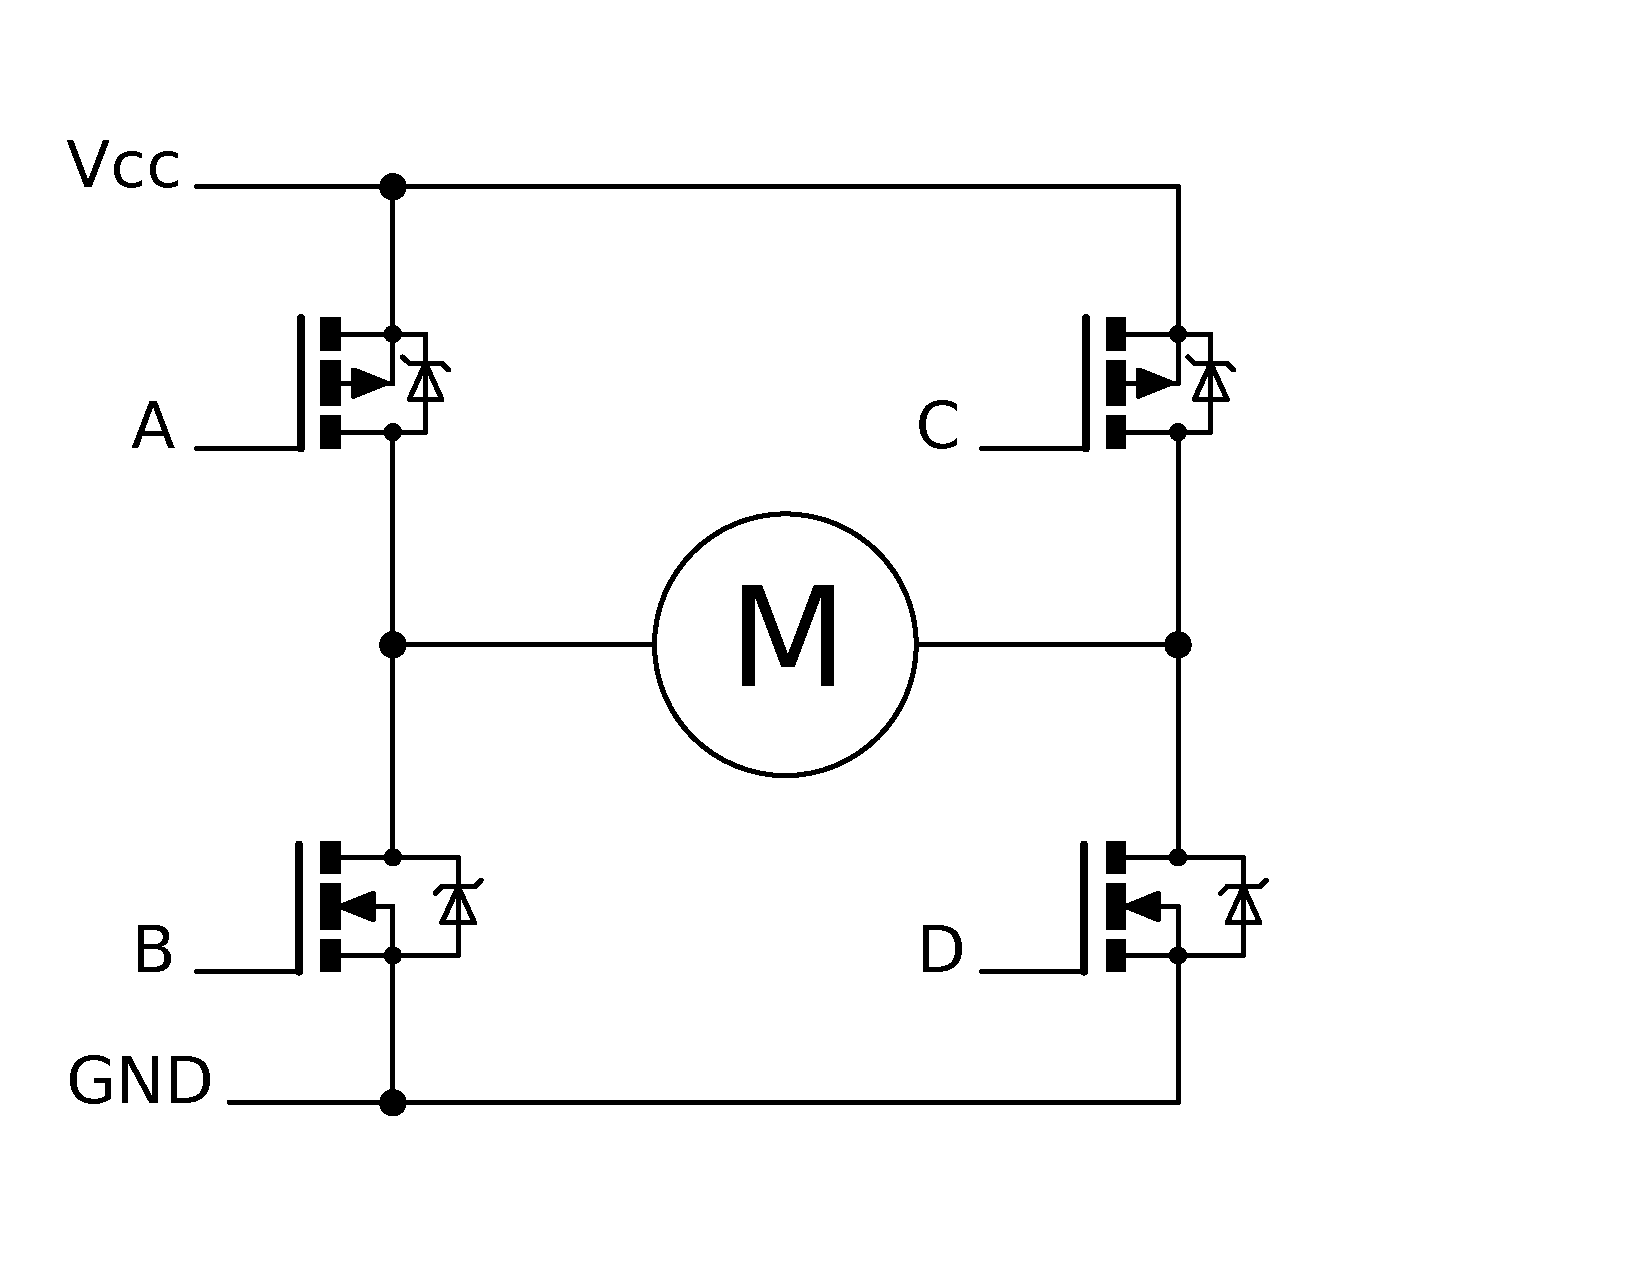
\includegraphics[width=0.8\textwidth]{pictures/hbrigde.pdf}
  \caption{Diagram over simpel H-bro}
  \label{fig:hbro}
\end{figure}

H-broen på Swagwayen er lidt mere kompleks. Hele logikken kan findes på tabel \ref{tab:sandhed}. 
\section{PWM}
Pulsbreddemodulation (Pulse-Width-Modulation): Er en metode til at kontrollere spændingen i elektriske
apparater. Det er en metode til at levere spænding igennem en række impulser i stedet for der konstant er strøm igennem systemet. Ved at øge eller formindske bredden af impulsen kan man kontrollere en motor.

Man kan altså sige, at PWM er et on/off system hvor man styrer ved hurtigt, at slukke og tænde for
spændingen. Tiden der går imellem at den er on/off er så kort, at en LED som sådan ikke mærker det. Så
den vil ikke blinke, men derimod lyse mindre hvis man øger bredden imellem impulserne.

Måden vi styre dette på i en Arduino er via \texttt{analogWrite(pin,\dots);}. Her har vi mulighed for at give en værdi fra 0--255. Dette betyder at \texttt{analogWrite(pin,255);} er 100\% og \texttt{analogWrite(pin,127);} er 50\%. Dette kan også ses på figur \ref{fig:pwm}.\fxwarning{Hele afsnittet skal omskrives}
\begin{figure}[htbp]
  \centering
  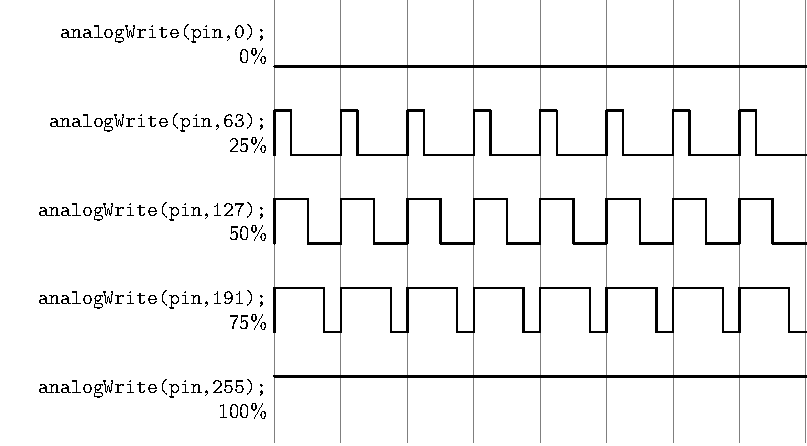
\includegraphics[width=\textwidth]{pictures/pwm.pdf}
  \caption{Eksempel på PWM med varierende dutycycle}
  \label{fig:pwm}
\end{figure}

\section{Overvejelser}
Der er to muligheder under fremstilling af en H-bro. Enten kan der benyttes en simpel H-bro chip, eller man kan fremstille en selv. Chippen er den nemme løsning, som gør alting super let at arbejde med. Dog kan chippen ikke håndtere store strømme, og det var derfor urealistisk at piggy-back dem.

Vi fremstillede derfor selv en H-bro, da den kan klare de store mængder af strøm vi arbejder med, selvom at det er langt mere komplekst og det forøger kraftigt mængden af ting der kan gå galt.

Efter som at motorene skal kunne køres med variable hastigheder, skal der køres PWM på disse. Man kan vælge, om dette skal ske i toppen eller bunden af H-broen som diskuteret før \ref{sec:H-broen}. Vi startede med at gøre dette i toppen, men dette blev senere ændret til bunden, hvilket er dybere beskrevet i motorcontroller v2.1. \ref{sec:Motorcontroller2.1}
\section{Motorcontroller}

\begin{table}[htbp]
  \caption{Motorcontroller v5.2 sandhedstabel}
  \centering
  % \begin{threeparttable}
  \begin{tabular}{ccc|cccc|ccccl}
    \toprule
    \multicolumn{3}{c}{Arduino pin}&\multicolumn{4}{c}{HEXFET spænding}&\multicolumn{4}{c}{HEXFET on/off}\\
    P7&P6&P5 &Q1&Q2&Q3&Q4 &Q1&Q2&Q3&Q4\\
    P8&P9&P10 &Q5&Q6&Q7&Q8 &Q5&Q6&Q7&Q8\\
    \midrule
    0&0&0 &0&1&0&0 &0&0&0&1 & Off ($\circlearrowright$)\\
    1&0&0 &0&0&0&1 &0&1&0&0 & Off ($\circlearrowleft$)\\
    0&1&0 &1&1&0&0 &1&0&0&1 & $\circlearrowright$\\
    1&1&0 &1&0&0&1 &1&1&0&0 & Short\\
    0&0&1 &0&1&1&0 &0&0&1&1 & Short\\
    1&0&1 &0&0&1&1 &0&1&1&0 & $\circlearrowleft$\\
    0&1&1 &1&1&1&0 &1&0&1&1 & Short\\
    1&1&1 &1&0&1&1 &1&1&1&0 & Short\\
    \bottomrule
  \end{tabular}
  % \begin{tablenotes}
  % \end{tablenotes}
  % \end{threeparttable}
  \legend{Tabellen viser hvordan den seneste motorcontroller, v5.2, opføre sig hvis den får inputtet angivet under “Arduino Pin”}
  \label{tab:sandhed}
\end{table}

H-bro, PWM, PWM-kondensator, beskyttelses dioder, 4000 serie, optocopler

\subsection{Samlet board}
Det var upraktisk at have alle funktioner på samme board. H-broerne og optocouplerne blev flyttet på sit eget board “Motorcontroller v1.0”.

\subsection{Motorcontroller v1.0}
\boarddate{24. januar 2012}
\fxwarning{Indsæt diagram over Motorcontroller v1.0}
\fxwarning{Indsæt figur over Motorcontroller v1.0}
\subsubsection{Det var der galt}
Boardet virkede ikke. Det opførte sig som det var kortsluttet. Det viste sig, at efter boardet var skilt helt af igen, at det plus tegn der skulle vise polariteten var sat ved den forkerte pol. Printet havde taget skade af at blive loddet på flere gange.

Der var desuden nogle af ledningene for tætsiddene og loddeøerne var lidt underdimensionerede. Der manglede også en mulighed for at se, hvilken vej strømmen løber i H-broerne.
\subsubsection{Det blev der rettet}
Plus tegnet blev flyttet over til den rigtige pol. Ledningerne blev flyttet længere væk fra hinanden, og loddeøernes størrelser forøget.

\subsection{Motorcontroller v2.0}
\boarddate{8. marts 2012} 
\subsubsection{Det var der galt}
Dette board blev aldrig lavet færdigt; Ledningerne omkring pinheaderen var for tæt efter at loddeøeren blev forstørret. Diagram og figur over printet kan findes i bilag. \fxwarning{ref}

\subsubsection{Det blev der rettet}
Loddeøerne blev gjort en smule mindre for at tillade ledningerners forbipasserend.
\subsection{Motorcontroller v2.1}
\boarddate{8 marts 2012}
\begin{figure}[htbp]
  \centering
  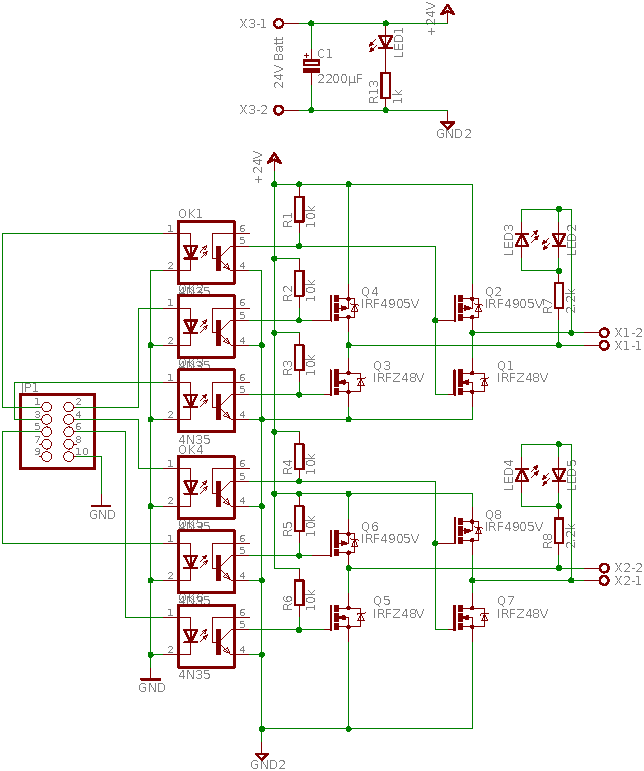
\includegraphics[width=\textwidth]{pictures/MotorcontrollerSch2-1.pdf}
  \caption{Diagram over Motorcontroller v2.1}
  \label{fig:mosch2.1}
\end{figure}
\subsubsection{Det var der galt}
\label{sec:Motorcontroller2.1}
\fxwarning{ref til fig:mosch2.1}
Boardet fungerede umiddelbart. Motoren kunne køre i begge retninger og farten kunne styres med PWM. Dog startede motoren på ca. 30\% fart uintentionelt i den ene retning. Ved at måle på PWM signalet fra mainboardet og signalet til motoren via. et oscilloskop, kunne problemet indskrænkes til at være på Motorcontrolleren.

Det viste sig efter megen debugging, at spændingen på gaten på P-kanal HEXFETerne (IRF4905) ikke gik \texttt{HIGH} lige så hurtigt som ventet. Der blev opstillet et forsøg på et breadboard med en P-kanal HEXFET, en optocoupler og en Arduino, for at gennemskue problemet.

\fxwarning{Indsæt diagram over forsøg med optocoupler og HEXFET}

Forsøget viste, at når optocoupleren sad mellem HEXFETen og Arduinoen var der en ubekendt kapacitet mellem HEXFETens gate og source. Figur \ref{fig:stigetid} viser nederst PWM signalet fra Arduinoen og øverst signalet på P-kanal HTXFETens gate, hvor man tydeligt kan se, at det tager en ubelejlig tid før signalet på gaten stiger.
\begin{figure}[htbp]
  \centering
  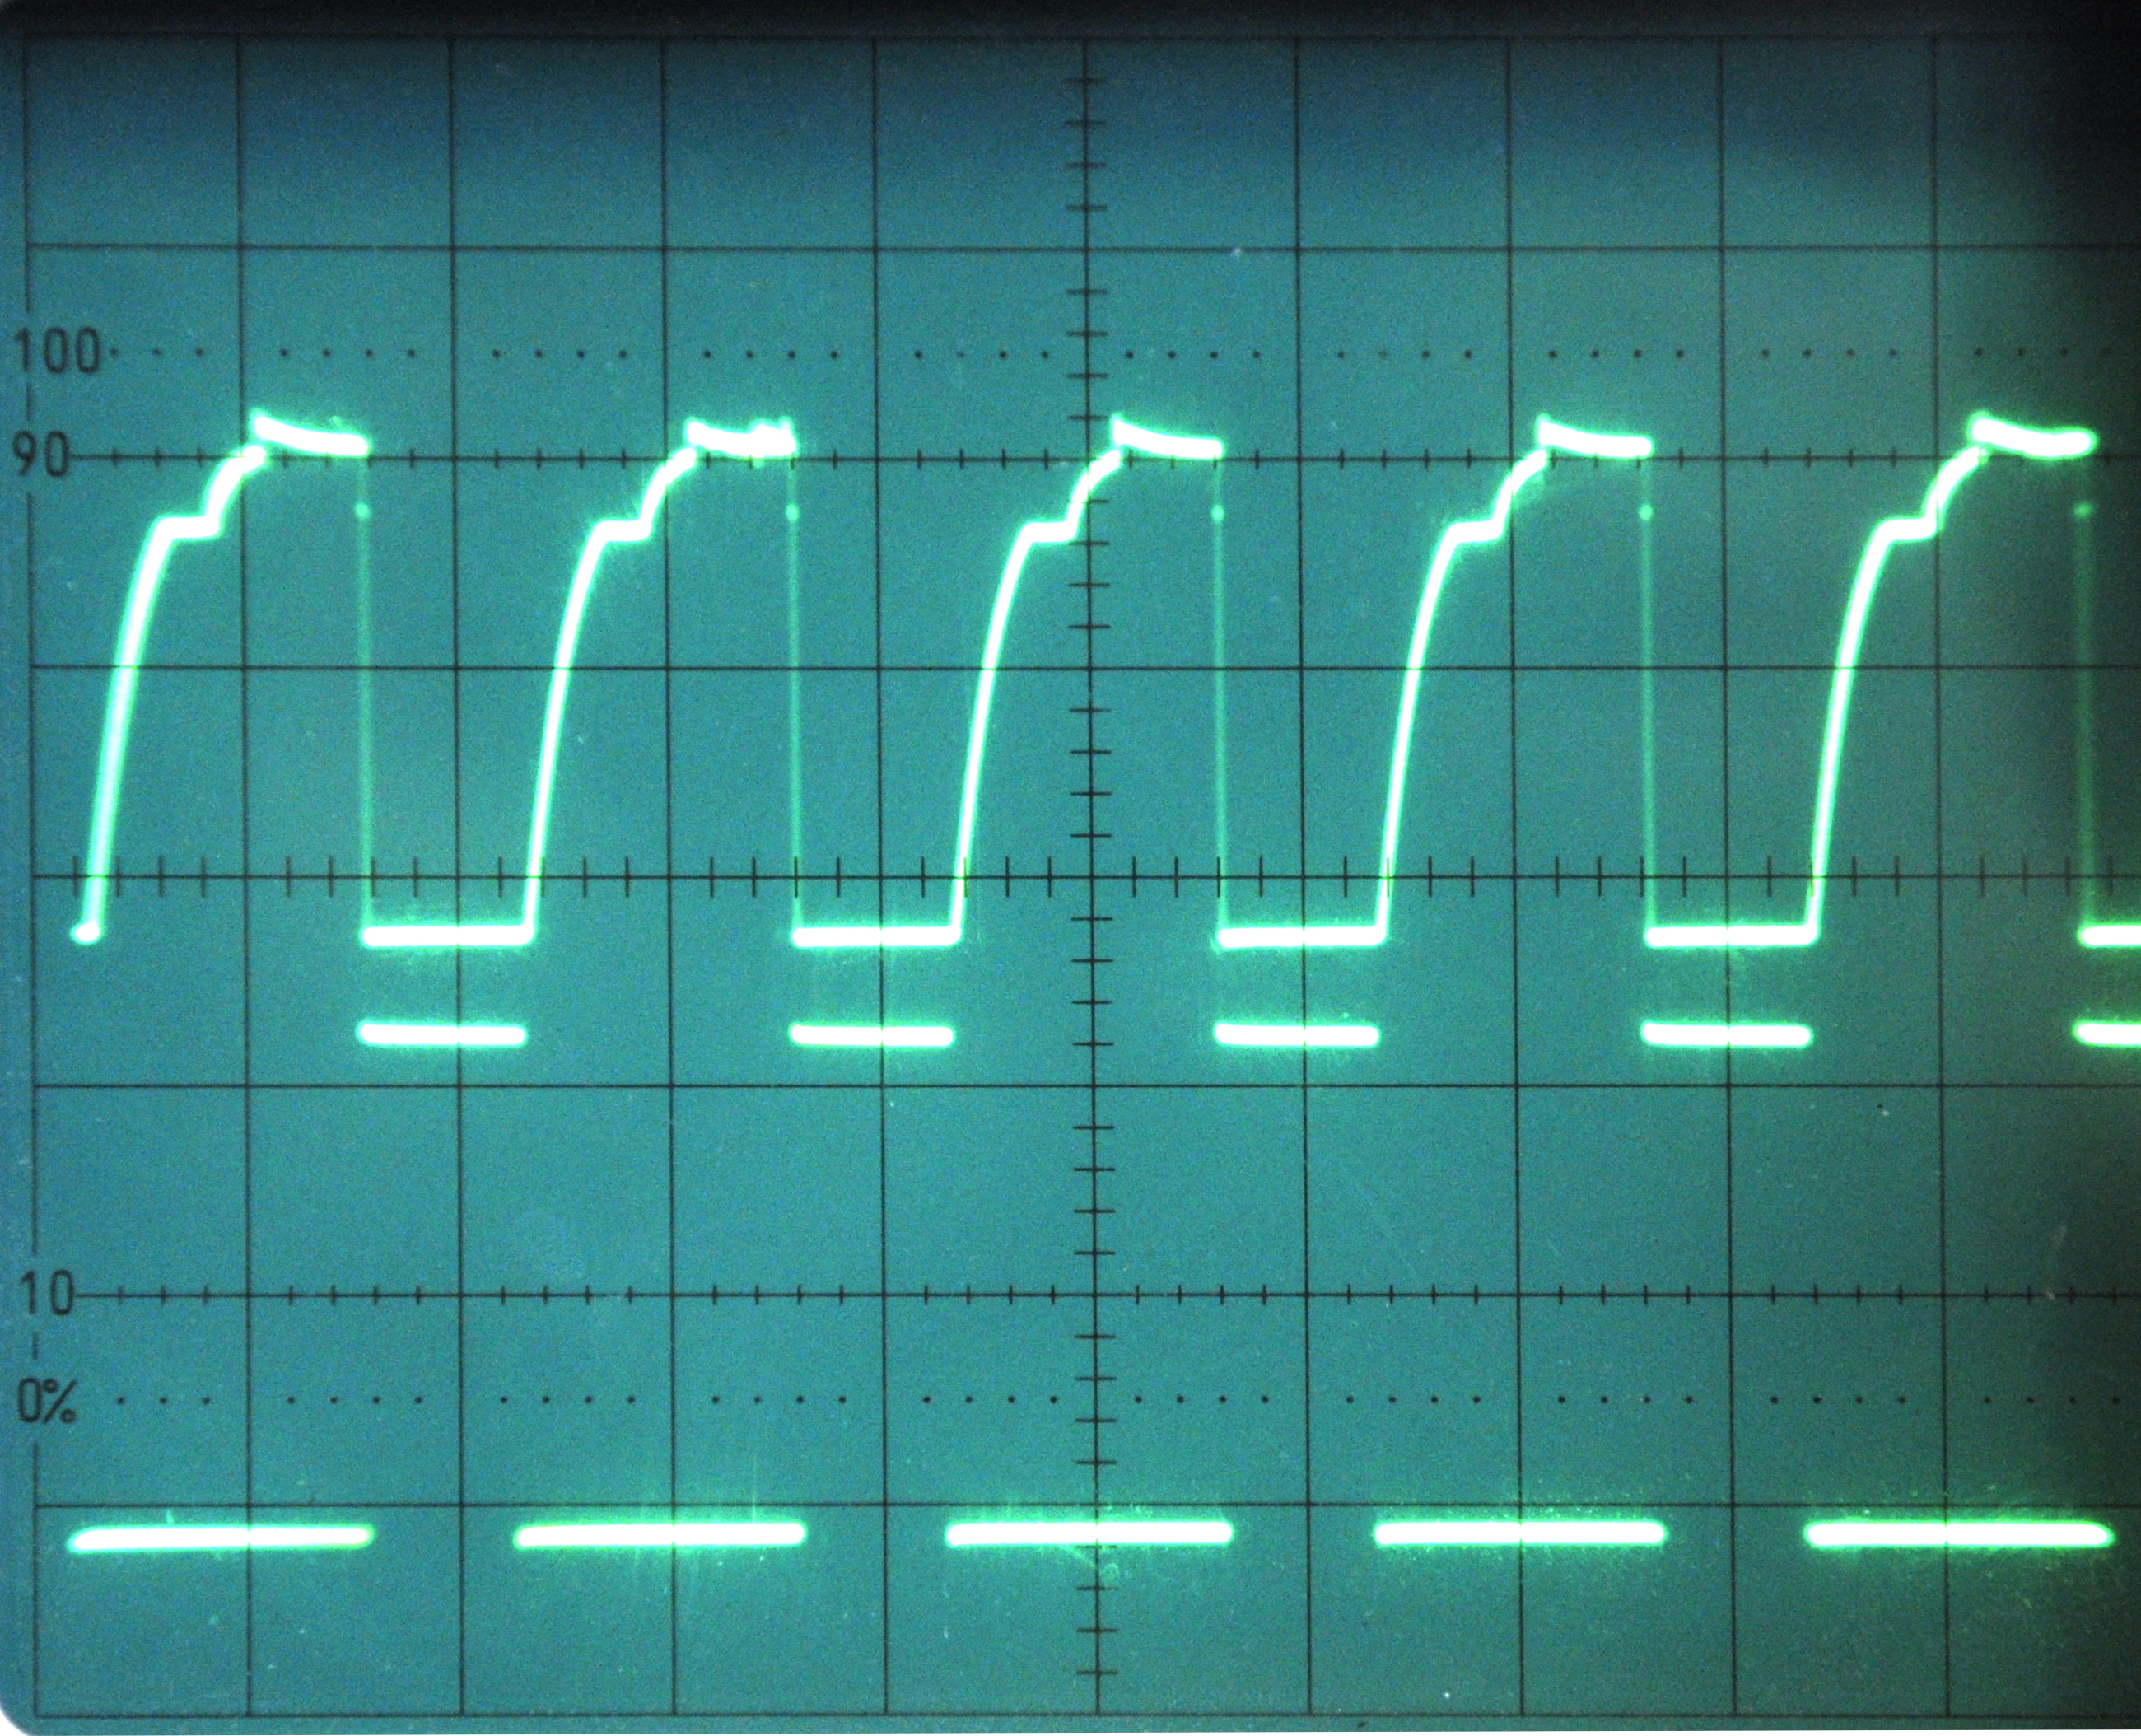
\includegraphics[width=0.8\textwidth]{pictures/stigetid.jpg}
  \caption[Oscilloskop billede af stigetid på en P-kanal HEXFET gate]{Oscilloskop billede af stigetid på en P-kanal HEXFET gate. Nederst ses PWM-signalet fra Arduinoen, øverst ses signalet på HEXFETens gate.}
  \label{fig:stigetid}
\end{figure}

Ved at sætte en mindre pull-up modstand på, kunne gaten aflades hurtigere, men det var ikke muligt at få den tilpas langt ned til at kunne styre motoren godt. Ved at fjerne optocoupleren og køre HEXFETens gate direkte fra Arduinoen eller ved fjerne HEXFETen og måle direkte på optocoupleren, var stigningstiden $\approx0$. Det var kun i kombination mellem HEXFETen og transistoren i optocoupleren, at stigningstiden ikke var $\approx0$.

Der blev forsøgt med en 4N25 optocoupler istedet for 4N35, og en BC547 istedet for optocoupleren; der var samme stigningstid.

Det har ikke været muligt, selv med hjælp fra vejleder, at forklare hvorfor denne kapacitet er der.

Problemet blev ikke løst, det blev bare gjort ubetydeligt: Istedet for at bruge en N- og en P-kanal HEXFET til at bestemme retning og køre PWM på de andre to N- og P-kanal HEXFETer, blev det lavet om til at begge P-kanal HEXFETer blev brugt til at bestemme retning og at N-kanal HEXFETerne bliver brugt at køre PWM. Det er ikke et problem at stigetiden på P-kanal HEXFETerne er langsom da de kun ændre sig når der skiftes retning og ikke med høj frekvens som ved PWM.

For ikke at tilføje flere optocouplere og bruge flere pins på Arduinoen blev der, på motorcontrolleren tilføjet to invertere.
\subsubsection{Det blev der rettet}
Vi byttede om på to P- og N-kanal HEXFETer, så der nu køres PWM på N-kanalen, og P-kanalen bestemmer retning. Derudover blev det tilføjet to invertere på motorcontrolleren. Se figur \fxwarning{ref: dia:v3.0}

\subsection{Motorcontroller v3.0}
\boarddate{27. marts 2012}
\subsubsection{Det var der galt} 
\fxwarning{Indsæt diagram over Motorcontroller v3.0 (Figur over printet kan findes i bilag)}
Efter at der blev tilføjet en inverter på to af gatesne til P-kanal HEXFETerne er denne \texttt{LOW} når der ikke er spænding på optocouplerne (for eksempel når den ikke er koblet til mainboardet). Det tænder HEXFETen sammen med N-kanal HEXFETerne, som også er tændt uden spænding på optocouplerne, hvilket kortslutter H-broen. Motorcontroller v3.0 var fungerede, men det var upraktisk, at den var kortsluttet uden at være koblet sammen med mainboardet.

\subsubsection{Det blev der rettet}
Pull-up modstandende blev derfor erstattet med pull-down modstande.
\subsection{Motorcontroller v4.0}
\boarddate{12. april 2012} 
\subsubsection{Det var der galt} 
Dette board blev aldrig lavet færdigt. 
En stor del af boardet blev re-routed da der var blevet rodet efter mange versioner. Diagram og Figur over printet kan findes i bilag. \fxwarning{ref}
\subsubsection{Det blev der rettet}
Boardet blev rerouted pga. rod.
\subsection{Motorcontroller v4.1}
\boarddate{13. april 2012}
\subsubsection{Det var der galt} 
Der var en ledning der ikke var routed og der var noget mindre re-routing.
\subsubsection{Det blev der rettet}
Rettet op på fejl i routing
\subsection{Motorcontroller v4.2}
\boarddate{17. april 2012} 
\subsubsection{Det var der galt} 
Dette board blev aldrig lavet færdigt.
For-modstandene til optocouplerene sad på mainboardet af en ukendt årsag. Det virkede mere logisk og praktisk at have disse på motorboardet.
\subsubsection{Det blev der rettet}
For-modstandene til optocouplerne blev flyttet fra mainboardet til motorcontrolleren.
\subsection{Motorcontroller v5.0}
\boarddate{24. april 2012} 
\subsubsection{Det var der galt} 
Dette board blev aldrig lavet færdigt.
Det er svært at debugge motorcontrolleren når man ikke kan se hvad der sker. Optocouplerenes manglende tegn på hvad der sker skabte problemer.
\subsubsection{Det blev der rettet}
Der blev tilføjet LEDer til optocouplerne.
\subsection{Motorcontroller v5.1}
\boarddate{24. april 2012} 
\subsubsection{Det var der galt} 
Dette board blev aldrig lavet færdigt.
Logikken blev ændret pga. en fejl.
\subsubsection{Det blev der rettet}
Nogle ledninger i fladkablet blev byttet om.
\subsection{Motorcontroller v5.2}
\boarddate{24. april 2012}

\fxwarning{Board brænder af}
\begin{figure}[htbp]
  \centering
  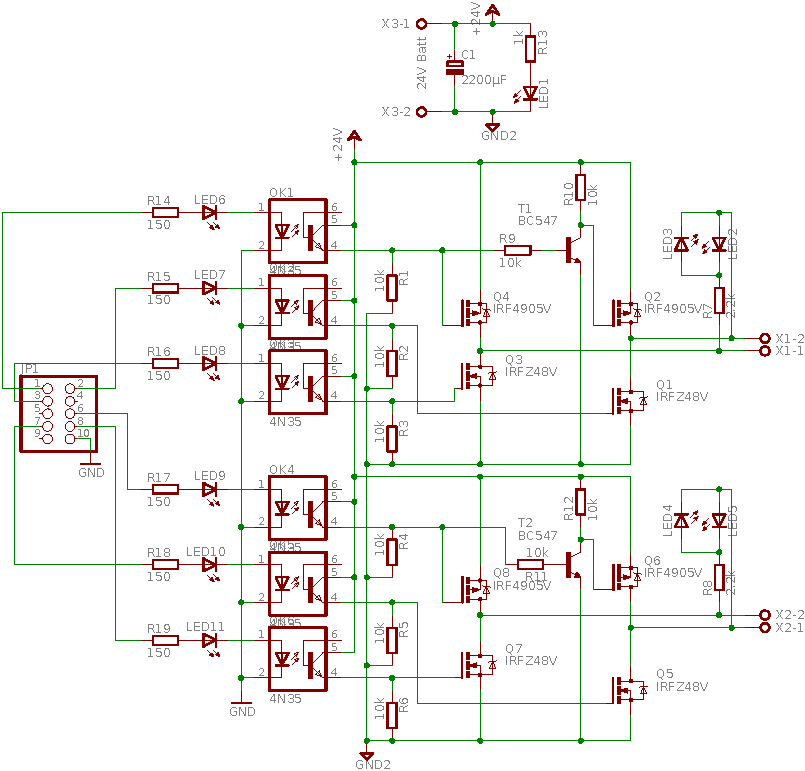
\includegraphics[width=\textwidth]{pictures/MotorcontrollerSch5-2.pdf}
  \caption{Diagram over Motorcontroller v5.2}
  \label{fig:mosch5.2}
\end{figure}
\fxwarning{ref til fig:mosch5.2}
\subsubsection{Det var der galt} 
Boardet v5.2 sidder i Swagway produktet og fungerer. Den nuværende version er en erstatning af et magen til, da dette brændte af under en længerevarende, ellers succesfuld, prøvekørsel.

Motorene danner strøm når de går i frigang, og hvis man derfor kører hurtigt fremad, og ændrer vinklen til et modsatgående fortegn, sendes strømmen tilbage igennem boardet. Der blev derfor tilføjet beskyttelses dioder for at tage strømmen.
\subsubsection{Det blev der rettet}
Der blev til v6.0 tilføjet beskyttelses dioder til kredsløbet, for at tage strømmen fra motorene.
\subsection{Motorcontroller v6.0}
\boarddate{24. april 2012}

\chapter{Auxiliary}
\begin{table}[htbp]
  \caption{Pin forbindelser på Arduino}
  \centering
  \begin{threeparttable}
    \begin{tabular}{rll}
      \toprule
      Pin & Forbindelse & Egenskaber\\
      \midrule
      0 & USB Rx & \\
      1 & USB Tx & \\
      2 & Radio Rx & Interrupt\\
      3 & & Interrupt, PWM\\
      4 & Radio Tx & \\
      5 & Motorcontroller R2 & PWM\tnote{a}\\
      6 & Motorcontroller L2 & PWM\tnote{a}\\
      7 & Motorcontroller L1 & \\
      8 & Motorcontroller R1 & \\
      9 & Motorcontroller L3 & PWM\\
      10 & Motorcontroller R3 & PWM\\
      11 & & PWM\\
      12 & & \\
      13 & & LED\\
      A0 & & \\
      A1 & & \\
      A2 & Steering & \\
      A3 & Steering & \\
      A4 & IMU I²C SDA & SDA\\
      A5 & IMU I²C SCL & SCL
    \end{tabular}
    \begin{tablenotes}
      \item[a]{PWM outputtet fra disse er lidt højere end forventet. De drives af en anden timer.\issue{42} Se under Mainboard 4.0 i sektion \ref{sec:main40}.}
    \end{tablenotes}
  \end{threeparttable}
  % \label{tab:}
\end{table}

\section{Mainboard}

\subsection{Mainboard v1.0}
\boarddate{24 jan 2012}
\subsubsection{Det var der galt}
Mainboardets loddeøer var underdimensioneret\issue{1}, hvilket betyder, at lodninger blev besværlige. Yderligere var det ikke til at komme til at trykke på resetknappen på Arduinoen, da shieldet dækkede over knappen.\issue{2} 
\subsubsection{Det blev der rettet}
Der blev tilføjet en reset knap på mainboardet, i den følgende version. Der blev også tilføjet et stik til datamodtagning fra styringen på mainboardet.\issue{12}
Derudover blev loddeøerne udvidet.
\subsection{Mainboard v2.0}
\boarddate{1 marts 2012}
\subsubsection{Det var der galt}
Logik kredsløbet blev kasseret. Efterfølgende blev der brugt tre Arduino pins per motor.\issue{21} Display-boardet blev ligeledes kasseret.\issue{9} Pinheaderne til 9V og IMUen var desuden for tæt sammen.\issue{13}
\subsubsection{Det blev der rettet}
Pinheader til 9V batteri og IMU blev flttet længere væk fra hinanden. Nyt logik implementeret.
\subsection{Mainboard v3.0}
\boarddate{26 marts 2012} 
\subsubsection{Det var der galt}
Dette board blev aldrig lavet færdig.
På boardet blev der dog tilføjet pins til en radio, hvis formål er at kunne ændre reguleringsværdierne trådløst.\issue{29}
\subsubsection{Det blev der rettet}


\subsection{Mainboard v3.1}
\boarddate{29 marts 2012}
\subsubsection{Det var der galt}
For-modstandene var placeret på mainboardet, hvilket var ulogisk.\issue{37}
Pinheader til IMU passer med en 5×2 socket, men der er placeret en 7×2 på boardet.
\subsubsection{Det blev der rettet}
For-modstandene blev flyttet fra mainboardet til motorcontrolleren. Pinheaderen til IMUen blev lavet om.
\subsection{Mainboard v4.0}\label{sec:main40}
\boarddate{24 april 2012}
\subsubsection{Det var der galt}
Swagwayen kører med dette board, men den ene motor kørte hurtigere end den anden.\issue{42} Det lignede umiddelbart en mekanisk fejl, men ved at bytte om på ledningerne til motorene viste det sig at den ene kanal på motorcontrolleren kørte langsommere end den anden. 
Problement blev isoleret til, at Arduinoen ikke sendte PWM med samme frekvens til begge kanaler. I Arduino referencen for \texttt{AnalogWrite()} ser man også, at pin 5 og 6 PWM kører fra en anden timer end de andre PWM pins. Tilfældigvis kørte den ene motor på begge af disse pins. 

\subsubsection{Det blev der rettet}
Pin 5 og 9 blev byttet så Swagwayen kører lidt hurtigere forlæns end baglæns, men med samme forskel på begge hjul.

Ombytningen af de to pins blev gjort ved at bryde kobberbanerne på printet og lodde to ledninger på, der blev ikke lavet et nyt board.

\chapter{Mekanik}
\fxerror{Skriv om Motorer, batterier, etc.}

\chapter{Konklusion} \label{chap:kon}
Vores mål var at lave en balance robot, hvor vi havde tilvalgt at lave styring til begge sider, hvis tiden rækkede til det.

Swagwayen fungerer som den står idag, og kan balancere på egen hånd. Det viste sig, at lave styring så den kunne dreje var i overkanten af hvad vi kunne nå inden for den givne tidsramme, hvori vi dog opfyldte vores minimumskrav. Swagwayen kan også køre frem og tilbage med en fører.

\chapter{Perspektivering} \label{chap:per}
Som nævnt i projektbeskrivelsen, ville vi gerne med mere tid, have haft implementeret styring til Swagwayen. 
\fxerror{her mangler noget}
Kraftigere motorer med mindre gearkasser.
Encodere

\clearpage
\listoftables
\listoffigures
\nocite{*}
\bibliographystyle{dk-apali} \bibliography{bib}
\clearpage \appendix

\chapter{Arbejdsdeling}
\fxerror{Tilføj arbejdsdeling}

\section{Udvikling}
\section{Praktisk}
\section{Skriftligt}

\chapter{Kildekode}

\section{\texttt{swagway.ino}}
\lstinputlisting{../Software/swagway/swagway.ino}
\section{\texttt{ADXL345.h}}
\lstinputlisting{../Software/swagway/ADXL345.h}
\section{\texttt{ADXL345.cpp}}
\lstinputlisting{../Software/swagway/ADXL345.cpp}

\chapter{Status log}

\section{13. marts}
Mainbord er fungerende. v2.0 af motorboardet er næsten færdig.

Kredsløbet uden om printne er næsten færdig.

Vi kan læse data fra IMUen og vi har et halvt implementert kalman-filter.

Efter kalmanfilteret fungere skal der implementeres PID med wrapper kode.

\end{document} 